% Source: graduate-coursework/Research/Papers/drafts/autonomous_dataset_generation/Autonomous_Maritime_Radar_Dataset_Generation.tex

\documentclass[border=4pt]{standalone}
\usepackage{algpseudocode}
\usepackage{amsmath, amssymb}
\usepackage{graphicx}
\usepackage{tikz}

\newcommand{\PlaceHolder}[2]{%
  \fbox{%
    \begin{minipage}[c][#2][c]{#1}
      \centering\small
      FIGURE PLACEHOLDER\\
      Replace with final artwork
    \end{minipage}%
  }%
}

\begin{document}
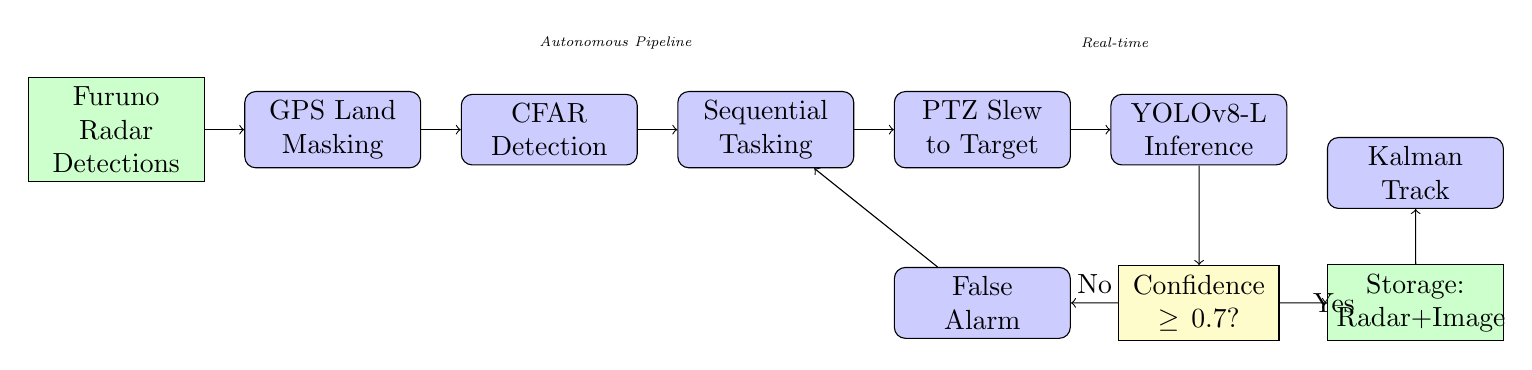
\begin{tikzpicture}[node distance=3cm, auto, scale=1.1]
  % Define styles
  \tikzstyle{block} = [rectangle, draw, fill=blue!20, text width=2cm, text centered, rounded corners, minimum height=0.8cm]
  \tikzstyle{decision} = [rectangle, draw, fill=yellow!20, text width=1.8cm, text centered, minimum height=0.9cm]
  \tikzstyle{io} = [rectangle, draw, fill=green!20, text width=2cm, text centered, minimum height=0.8cm]

  % Radar input
  \node[io] (radar) at (0,0) {Furuno Radar\\Detections};

  % Land masking
  \node[block] (masking) at (2.5,0) {GPS Land\\Masking};

  % CFAR detection
  \node[block] (cfar) at (5,0) {CFAR\\Detection};

  % Camera tasking
  \node[block] (tasking) at (7.5,0) {Sequential\\Tasking};

  % PTZ slew
  \node[block] (ptz) at (10,0) {PTZ Slew\\to Target};

  % YOLOv8 inference
  \node[block] (yolo) at (12.5,0) {YOLOv8-L\\Inference};

  % Decision
  \node[decision] (conf) at (12.5,-2) {Confidence\\$\geq 0.7$?};

  % False alarm path
  \node[block] (alarm) at (10,-2) {False\\Alarm};

  % Verified path
  \node[io] (storage) at (15,-2) {Storage:\\Radar+Image};

  % Kalman tracking
  \node[block] (kalman) at (15,-0.5) {Kalman\\Track};

  % Arrows
  \draw[->] (radar) -- (masking);
  \draw[->] (masking) -- (cfar);
  \draw[->] (cfar) -- (tasking);
  \draw[->] (tasking) -- (ptz);
  \draw[->] (ptz) -- (yolo);
  \draw[->] (yolo) -- (conf);
  \draw[->] (conf) -- node[above] {No} (alarm);
  \draw[->] (alarm) -- (tasking);
  \draw[->] (conf) -- node[right] {Yes} (storage);
  \draw[->] (storage) -- (kalman);

  % Add text annotations
  \node[text width=3cm, font=\tiny] at (6.25,1) {\textit{Autonomous Pipeline}};
  \node[text width=3cm, font=\tiny] at (12.5,1) {\textit{Real-time}};
\end{tikzpicture}
\end{document}
